
\section{実際の最終形態(卒論=pdf)への変換}
hiki+keynoteで卒論の内容ができたら,それを卒論の最終形態つまりpdfへ変換する必要が出てきます.

ここで問題が発生します.hikiよりもlatexの方が機能が豊富なこと.
つまり,簡易に書くにはhikiなどのmark downで書いていくのがいいんですが,
文書として完成度を高めるには,latexで細かい設定を調整する必要がどうしても出てきます.

具体的には,

\begin{enumerate}
\item 図の配置を調整するwrapの数値調整
\item 参照文献の記述
\item リスト,引用の体裁
\item 章立て階層構造
\end{enumerate}
などが問題になるところです.

これはhikiではどうしようもありません.一つの手はもう少し高機能なmark up言語
例えばasciidocなどに変更することですが,これはどこまでいっても終わりのない
方向のようで,結局はlatexで書いているのと同じになる可能性があります.

我々は違う戦略をとります.それは,
\begin{quote}\begin{verbatim}
latexをベースにして,hikiを生成する
\end{verbatim}\end{quote}
と言う手です.

DRY(Don't Repeat Yourself)原則さえ守れば,文書管理はいいのですから,
ある段階まですすめばhikiではなくlatexを原本にするのです.
そのための変換器latex2hikiとその派生rake環境が用意されています.
そちらはこちらで卒業後に変換します.参照文献はlatexに移してから
修正してください.

ここでは,hikiでできることをとことん突き詰めておきます.

\subsection{install}\begin{quote}\begin{verbatim}
hiki -i
\end{verbatim}\end{quote}
でinstallされています.新たに使うコマンド群は次の通りです.
\begin{quote}\begin{verbatim}
rake latex            # FILE1をlatexに変換
rake latex_all        # すべてのhikiファイルをlatex変換
rake latex_wrap       # FILE1をwrap formatでlatexに変換
rake reset_latex_dir  # latex_dirのゴミファイルを削除
\end{verbatim}\end{quote}
\subsection{rake latex(個別ファイルの変換)}\begin{quote}\begin{verbatim}
rake latex sync.hiki
\end{verbatim}\end{quote}
とすると,
\begin{quote}\begin{verbatim}
latex_dir/sync.tex
\end{verbatim}\end{quote}
にlatex変換後のファイルが生成します.これを,TeXShopでcommand\_t変換します.
完成例はこちらです.

\begin{itemize}
\item \verb|{{attach_anchor(sync.pdf,hikiutils_bob)}}|
\end{itemize}
うまくいかないときは,terminalで
\begin{quote}\begin{verbatim}
platex sync.tex
dvipdfmx sync.dvi
\end{verbatim}\end{quote}
を試してみてください.

\subsubsection{注意}
hikiの初めの部分は,
\begin{lstlisting}[style=customCsh,basicstyle={\scriptsize\ttfamily}]
bob% head -3 hikiutils_bob.hiki
! title:hikiutils -iによる卒論作成システム
! autor:Shigeto R. Nishitani
! date: Kwansei Gakuen Univ., 2017/1
\end{lstlisting}
とすると,
\begin{lstlisting}[style=customTeX,basicstyle={\scriptsize\ttfamily}]
\begin{document}
\title{hikiutils -iによる卒論作成システム}
\author{Shigeto R. Nishitani}
\date{ Kwansei Gakuen Univ., 2017/1}
\maketitle
\end{lstlisting}
と変換してくれます.次節のlatex\_allでは,basename.hikiに書かれたそれらの情報は,
head.texでtitleなどを用意するべきなので,自動で消されます.

必要な図は,figsから自動で取るようになっていますが,
サイズや解像度が問題のときは手動で調整してください.

\subsection{rake latex\_all手順(ディレクトリー内の一括変換)}
pwdのdirectoryと同名のbasenameに.hikiの拡張子がついたファイルが用意されていて,
\begin{quote}\begin{verbatim}
rake latex_all
\end{verbatim}\end{quote}
をおこなうと自動で全部を一体にまとめた文書へのlatex変換が出来上がります.
たとえば,hikiutils\_bob.hikiの記述を
\begin{lstlisting}[style=customCsh,basicstyle={\scriptsize\ttfamily}]
bob% cat hikiutils_bob.hiki 
!hikiutilsを用いた卒業論文作成

! [[hikiutils_bob_sync]]
! [[hikiutils_bob_latex_all]]

\end{lstlisting}
とすると,sync.tex, latex\_all.texがlatex\_dir内に変換されます.
さらに,開いているhikiutils\_bob.texをTeXShopで変換してみてください.

うまくできないときは\verb|ここ(http://qiita.com/hideaki_polisci/items/3afd204449c6cdd995c9)|を参照して自力で入れてみてください.だめならdonkey.

\begin{itemize}
\item \verb|{{attach_anchor(hikiutils_bob.pdf,hikiutils_bob)}}|
\end{itemize}
というようになります.

\subsubsection{下準備}
latex\_dir内に幾つかのtex雛形を入れておく必要があります.
\begin{quote}\begin{verbatim}
hiki -i
\end{verbatim}\end{quote}
とhikiutils環境を再度初期化すると,自動でインストールする設定です.
なかったら手動で作ってください.Rakefile以外は上書きしません.
また,latex\_dir/head.texは下に記す修正が必要です.

\paragraph{head.tex}
題目,学生番号,氏名を変更する.年月をチェック.
\\setcounter\{tocdepth\}はtocをどこまで表示するかのレベルに対応します.
原稿作成時は階層がわかりやすいように深めにしていますが,本番では2程度で十分です.
\begin{lstlisting}[style=customTeX,basicstyle={\scriptsize\ttfamily}]
bob% cat head.tex
\title{卒業論文\\
\vspace{4cm} hikiutilsを用いた\\卒業論文作成}
\author{ 関西学院大学 理工学部 情報科学科\\\\1234 西谷滋人}
\date{\vspace{3cm} 2017年  3月\\
\vspace{3cm} 指導教員  西谷 滋人 教授}
\maketitle
\setcounter{tocdepth}{6} %

\end{lstlisting}
\paragraph{pre.tex}
latex\_allのときは使っていません.formatedの時に読むようにしていますが...読めてないようです.いずれ調べます.

\paragraph{mainのpreamble部}
あまり変更しないほうがいいですが,いずれいじることになります.
例えば,フォントポイント数を12から10ptに変えるなどです.
\begin{lstlisting}[style=customTeX,basicstyle={\scriptsize\ttfamily}]
\documentclass[12pt,a4paper]{jsarticle}
\usepackage[dvipdfmx]{graphicx}
\usepackage[dvipdfmx]{color}
\usepackage{listings,jlisting}% to use japanese correctly, install jlistings.
\lstset{
  basicstyle={\small\ttfamily},
  identifierstyle={\small},
  commentstyle={\small\itshape\color{red}},
  keywordstyle={\small\bfseries\color{cyan}},
  ndkeywordstyle={\small},
  stringstyle={\small\color{blue}},
  frame={tb},
  breaklines=true,
  numbers=left,
  numberstyle={\scriptsize},
  stepnumber=1,
  numbersep=1zw,
  xrightmargin=0zw,
  xleftmargin=3zw,
  lineskip=-0.5ex
}
\lstdefinestyle{customCsh}{
  language={csh},
  numbers=none,
}
\lstdefinestyle{customRuby}{
  language={ruby},
  numbers=left,
}
\lstdefinestyle{customTex}{
  language={tex},
  numbers=none,
}
\lstdefinestyle{customJava}{
  language={java},
  numbers=left,
}

\end{lstlisting}
\subsection{補助コマンドの解説}
\subsubsection{rake reset\_latex\_dir(latex\_dirのゴミ掃除)}
わかりやすいようにまとめたり,ファイルの名称を変更した時には,過去のtexファイルが残る.
それらを整理する時に使用.head.texだけをescapeしてrm -rfで消すので,注意が必要.
特に図形のfilesやbb filesは消えるので注意.

\subsubsection{wrap関係}
figure環境をwrapfigure環境で作るための幾つかのコマンド群です.
卒論ではfigure環境で作る方がいいんですが,journal論文などのページ数が制限された場合は,
wrapfigureでtextの回りこみや位置調整を行う必要があります.
それらのための環境を埋め込む仕組みです.

\begin{itemize}
\item rake change\_wrap(wrapで変換)
\item rake latex\_base(latexに変換するだけの下請け)
\item rake latex\_wrap(figure環境だけをwrapfig環境に変える)
\end{itemize}
Rakefile内の記述は
\begin{lstlisting}[style=customRuby,basicstyle={\scriptsize\ttfamily}]
desc "latex conversion FILE1"
task :latex => [:latex_base] do
  exit
end

desc "latex conversion FILE1 with wrap format"
task :latex_wrap => [:latex_base, :change_wrap] do
  exit
end
\end{lstlisting}
となっています.つまり,:latex\_baseをした後に,:change\_wrapを呼び出しています.

完成例はこちらです.

\begin{itemize}
\item \verb|{{attach_anchor(calphad_bob.pdf,hikiutils_bob)}}|
\end{itemize}
発表会の予稿ハンドアウトなどではこれが不可欠です.

\subsection{参照のシステム}
latexへ文献参照を渡すために,下記のようなフォーマットでの記述を行ってください.
\begin{lstlisting}[style=customCsh,basicstyle={\scriptsize\ttfamily}]
図{{ref(fig:SystemOverview)}}に卒論編集システムの概観を示しています.

!!!caption: (fig:SystemOverview)卒論編集システムの概観.
{{attach_view(hikiutils_bob.006.jpeg)}}

*基本的な使い方{{cite(listings1)}}
*独自のカラー化{{cite(listings2)}}
!reference:
:listings1:[[http://d.hatena.ne.jp/mallowlabs/20061226/1167137637]]
:listings2:[[http://www.ipc.akita-nct.ac.jp/~yamamoto/comp/latex/make_doc/source/source.html]]
\end{lstlisting}
\begin{itemize}
\item caption以下の丸括弧内にタグを書きます.
\item fig:以下のタグにsnake nameは使えません.Camelで書くようにしてください.
\item refでそれを参照します.
\item citeの方も同じです.
\item reference:以下の:...:記述がlatexではbibliographyに変わります.
\end{itemize}
これをsync, all\_latexをかけると図\ref{fig:CiteRefSystems}のようになります.latexの文献参照(cite, bibliography),図表番号の参照(ref, label)が正常に処理されていることが確認できます.また,web表示した場合でもそれほど違和感なく読めるでしょう.

\begin{figure}[htbp]\begin{center}
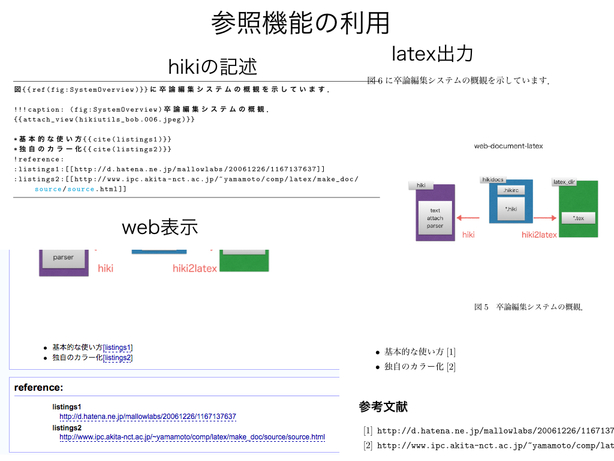
\includegraphics[width=10cm,bb= 0 0 737 553]{../figs/./hikiutils_bob.007.jpeg}
\caption{参照機能を利用した場合の変換後の表示.}
\label{fig:CiteRefSystems}
\label{default}\end{center}\end{figure}
